\chapter{\ChapterTitleScope}
\label{sec:zakres-funkcjonalnosci}


\section{Kontekst użytkowania aplikacji}

Głównym zadaniem aplikacji jest zapewnienie użytkownikom platformy
umożliwiającej rozgrywkę w~brydża. Strona internetowa aplikacji jest
przystosowana do każdego rozmiaru ekranu, z~której mógłby korzystać
użytkownik. Dzięki temu można skorzystać z~aplikacji, wykorzystując
telefon, komputer stacjonarny, laptop lub nawet telewizor. Wymagany
jest tylko dostęp do internetu.
%Aplikacja oprócz samej rozgrywki oferuje także przejrzenie
%wcześniejszych rozgrywek i~przeanalizowanie ich z~użyciem asystenta AI.

W~systemie aplikacji zdefiniowane są dwa typy użytkowników:
\begin{itemize}
  \item \textbf{zalogowany użytkownik} -- osoba posiadająca dostęp do
        funkcjonalności aplikacji,

  \item \textbf{anonimowy użytkownik} -- osoba niezalogowana, która nie
        posiada dostępu do
        % podstawowych
        funkcjonalności aplikacji.
        % Natomiast ma możliwość obserwowania trwających rozgrywek.
\end{itemize}

Funkcjonalności dostępne dla poszczególnych użytkowników:
\begin{itemize}
  \item \textbf{zalogowany użytkownik}:
        \begin{itemize}
          \item tworzenie i dołączanie do rozgrywek w brydża --
                gdy użytkownik założy lub zostanie jedynym
                użytkownikiem lobby, to staje się jego
                administratorem.
                Może zarządzać graczami znajdującymi się w~nim
                i~decydować ile graczy ma być zajęta przez asystenta AI.
          \item przeglądanie i analiza wcześniejszych rozgrywek
                z wykorzystaniem asystenta AI.
        \end{itemize}

  \item \textbf{anonimowy użytkownik}:
        \begin{itemize}
          \item obserwowanie trwających rozgrywek brydża.
        \end{itemize}
\end{itemize}

\begin{figure}[h]
  \centering
  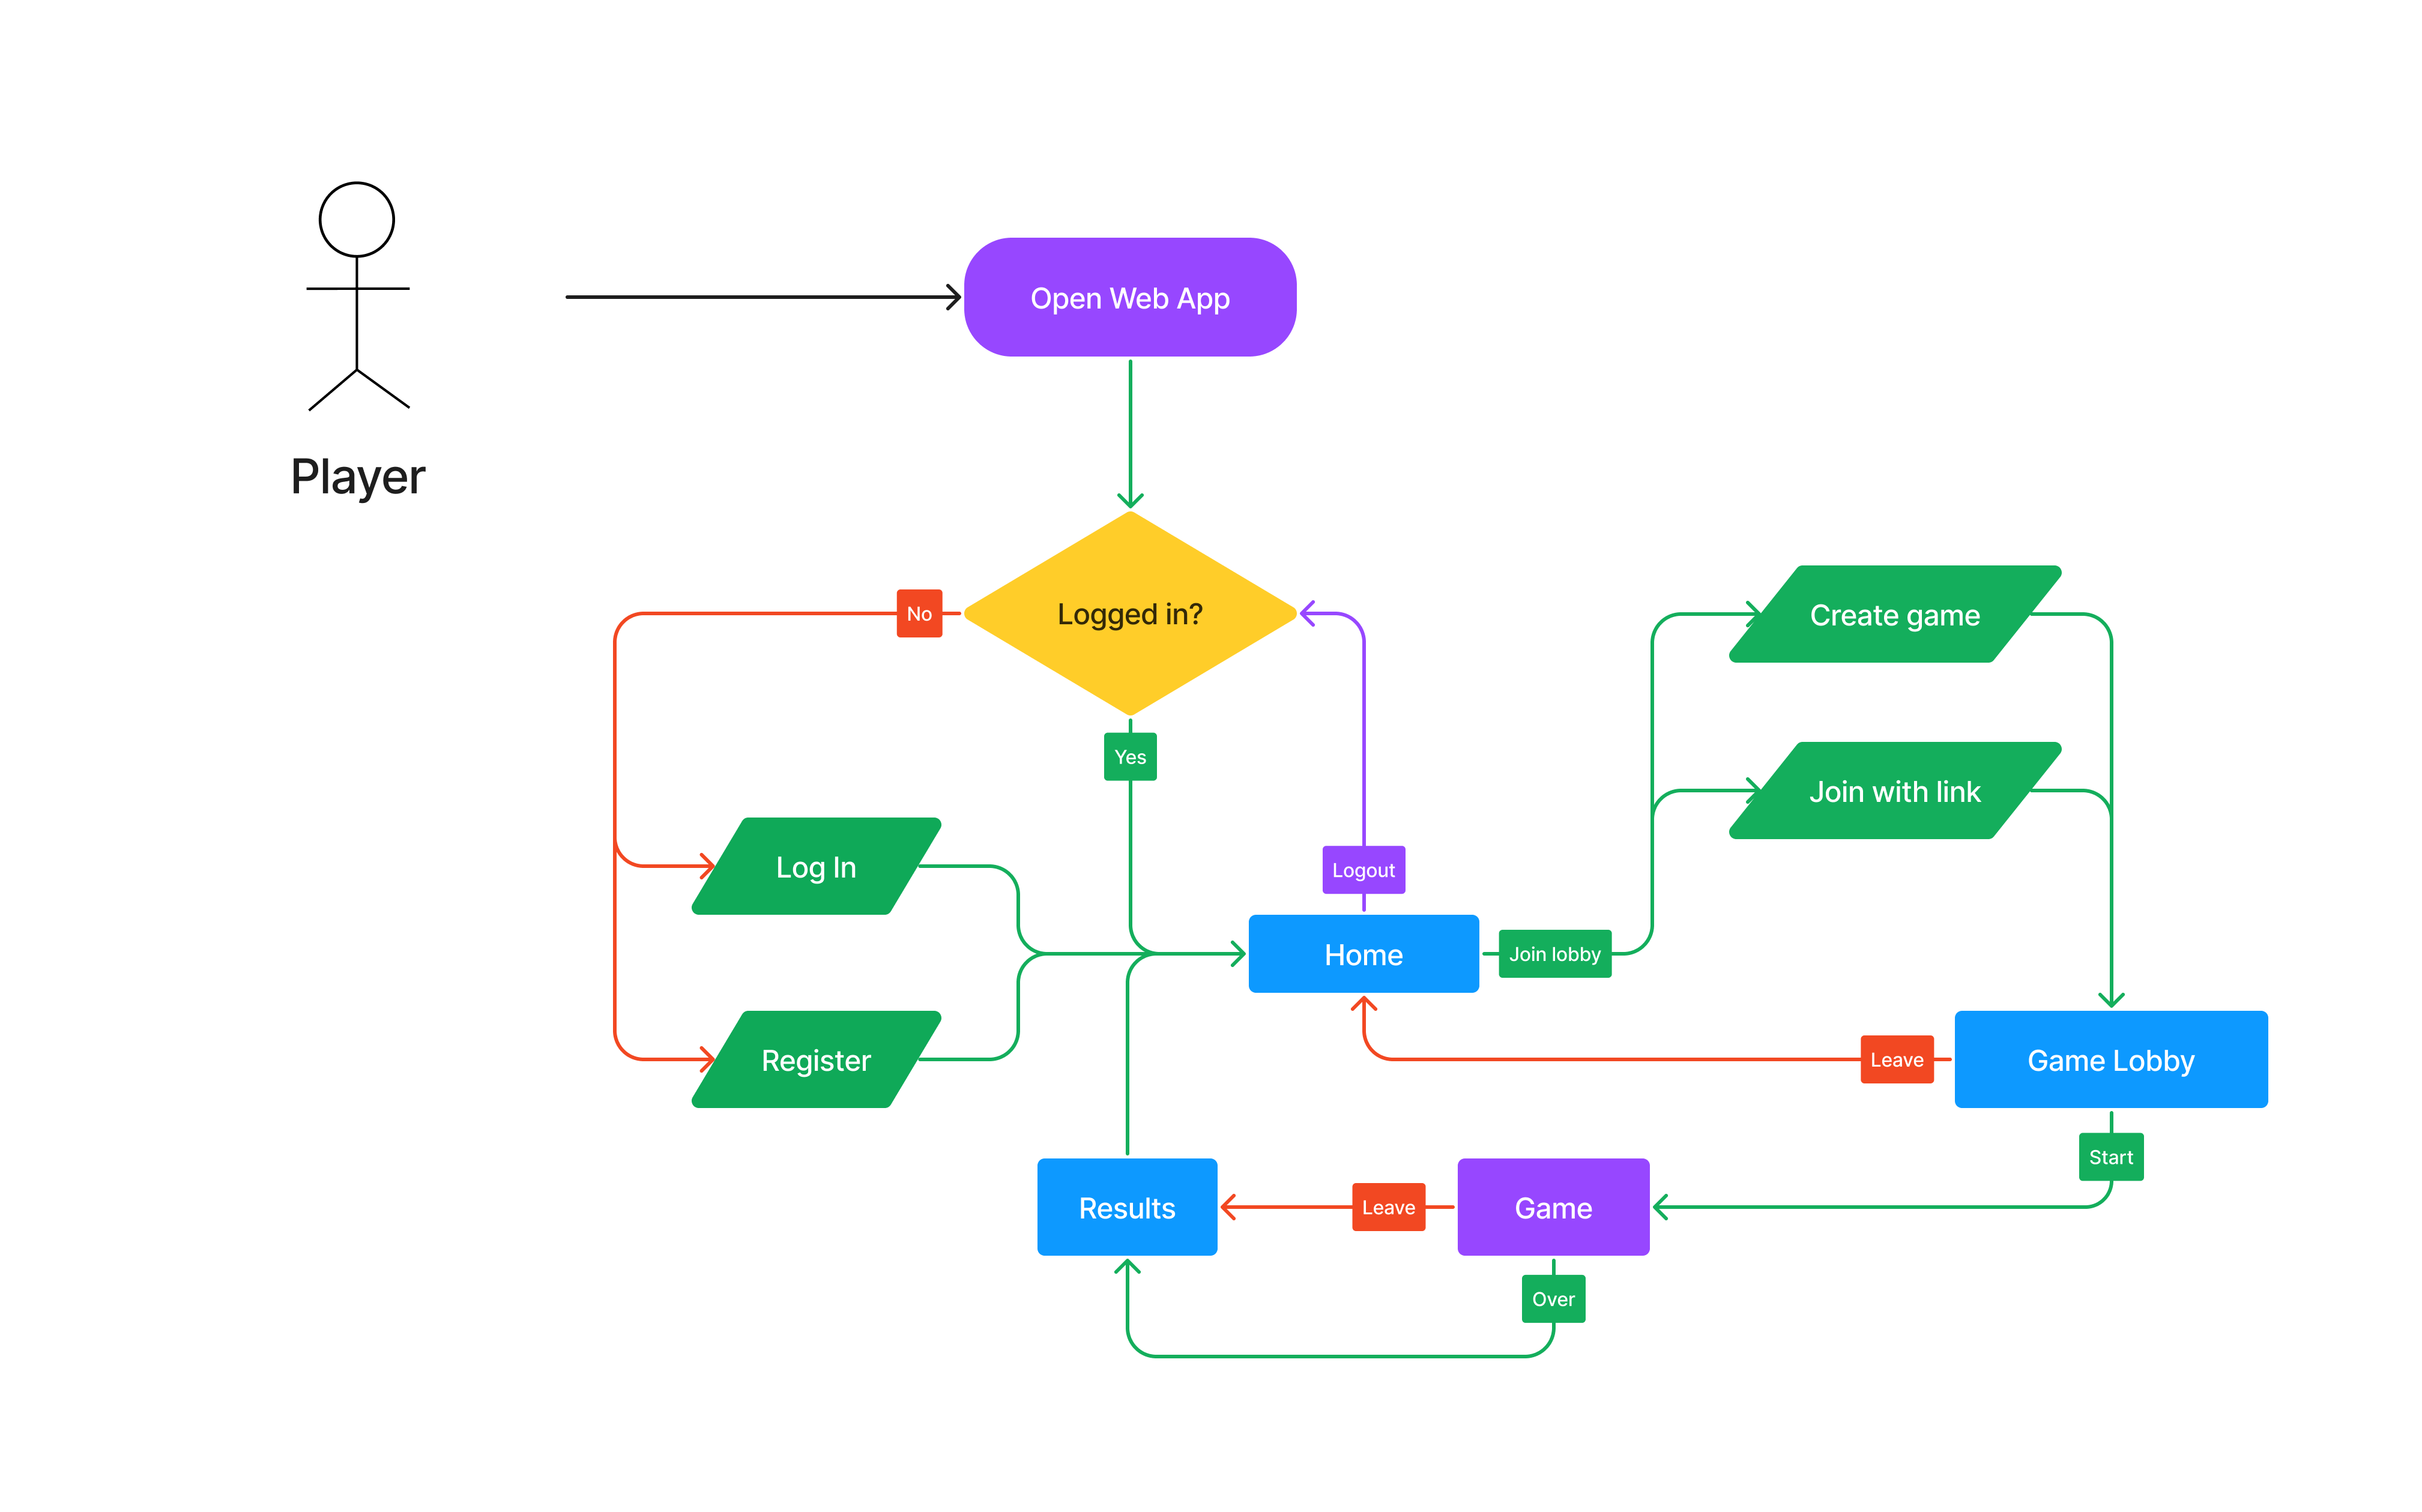
\includegraphics[width=\textwidth]{img/flow-aplikacji/user_flow.png}
  \caption{Schemat interakcji użytkownika z aplikacją}
\end{figure}

\begin{figure}[h]
  \centering
  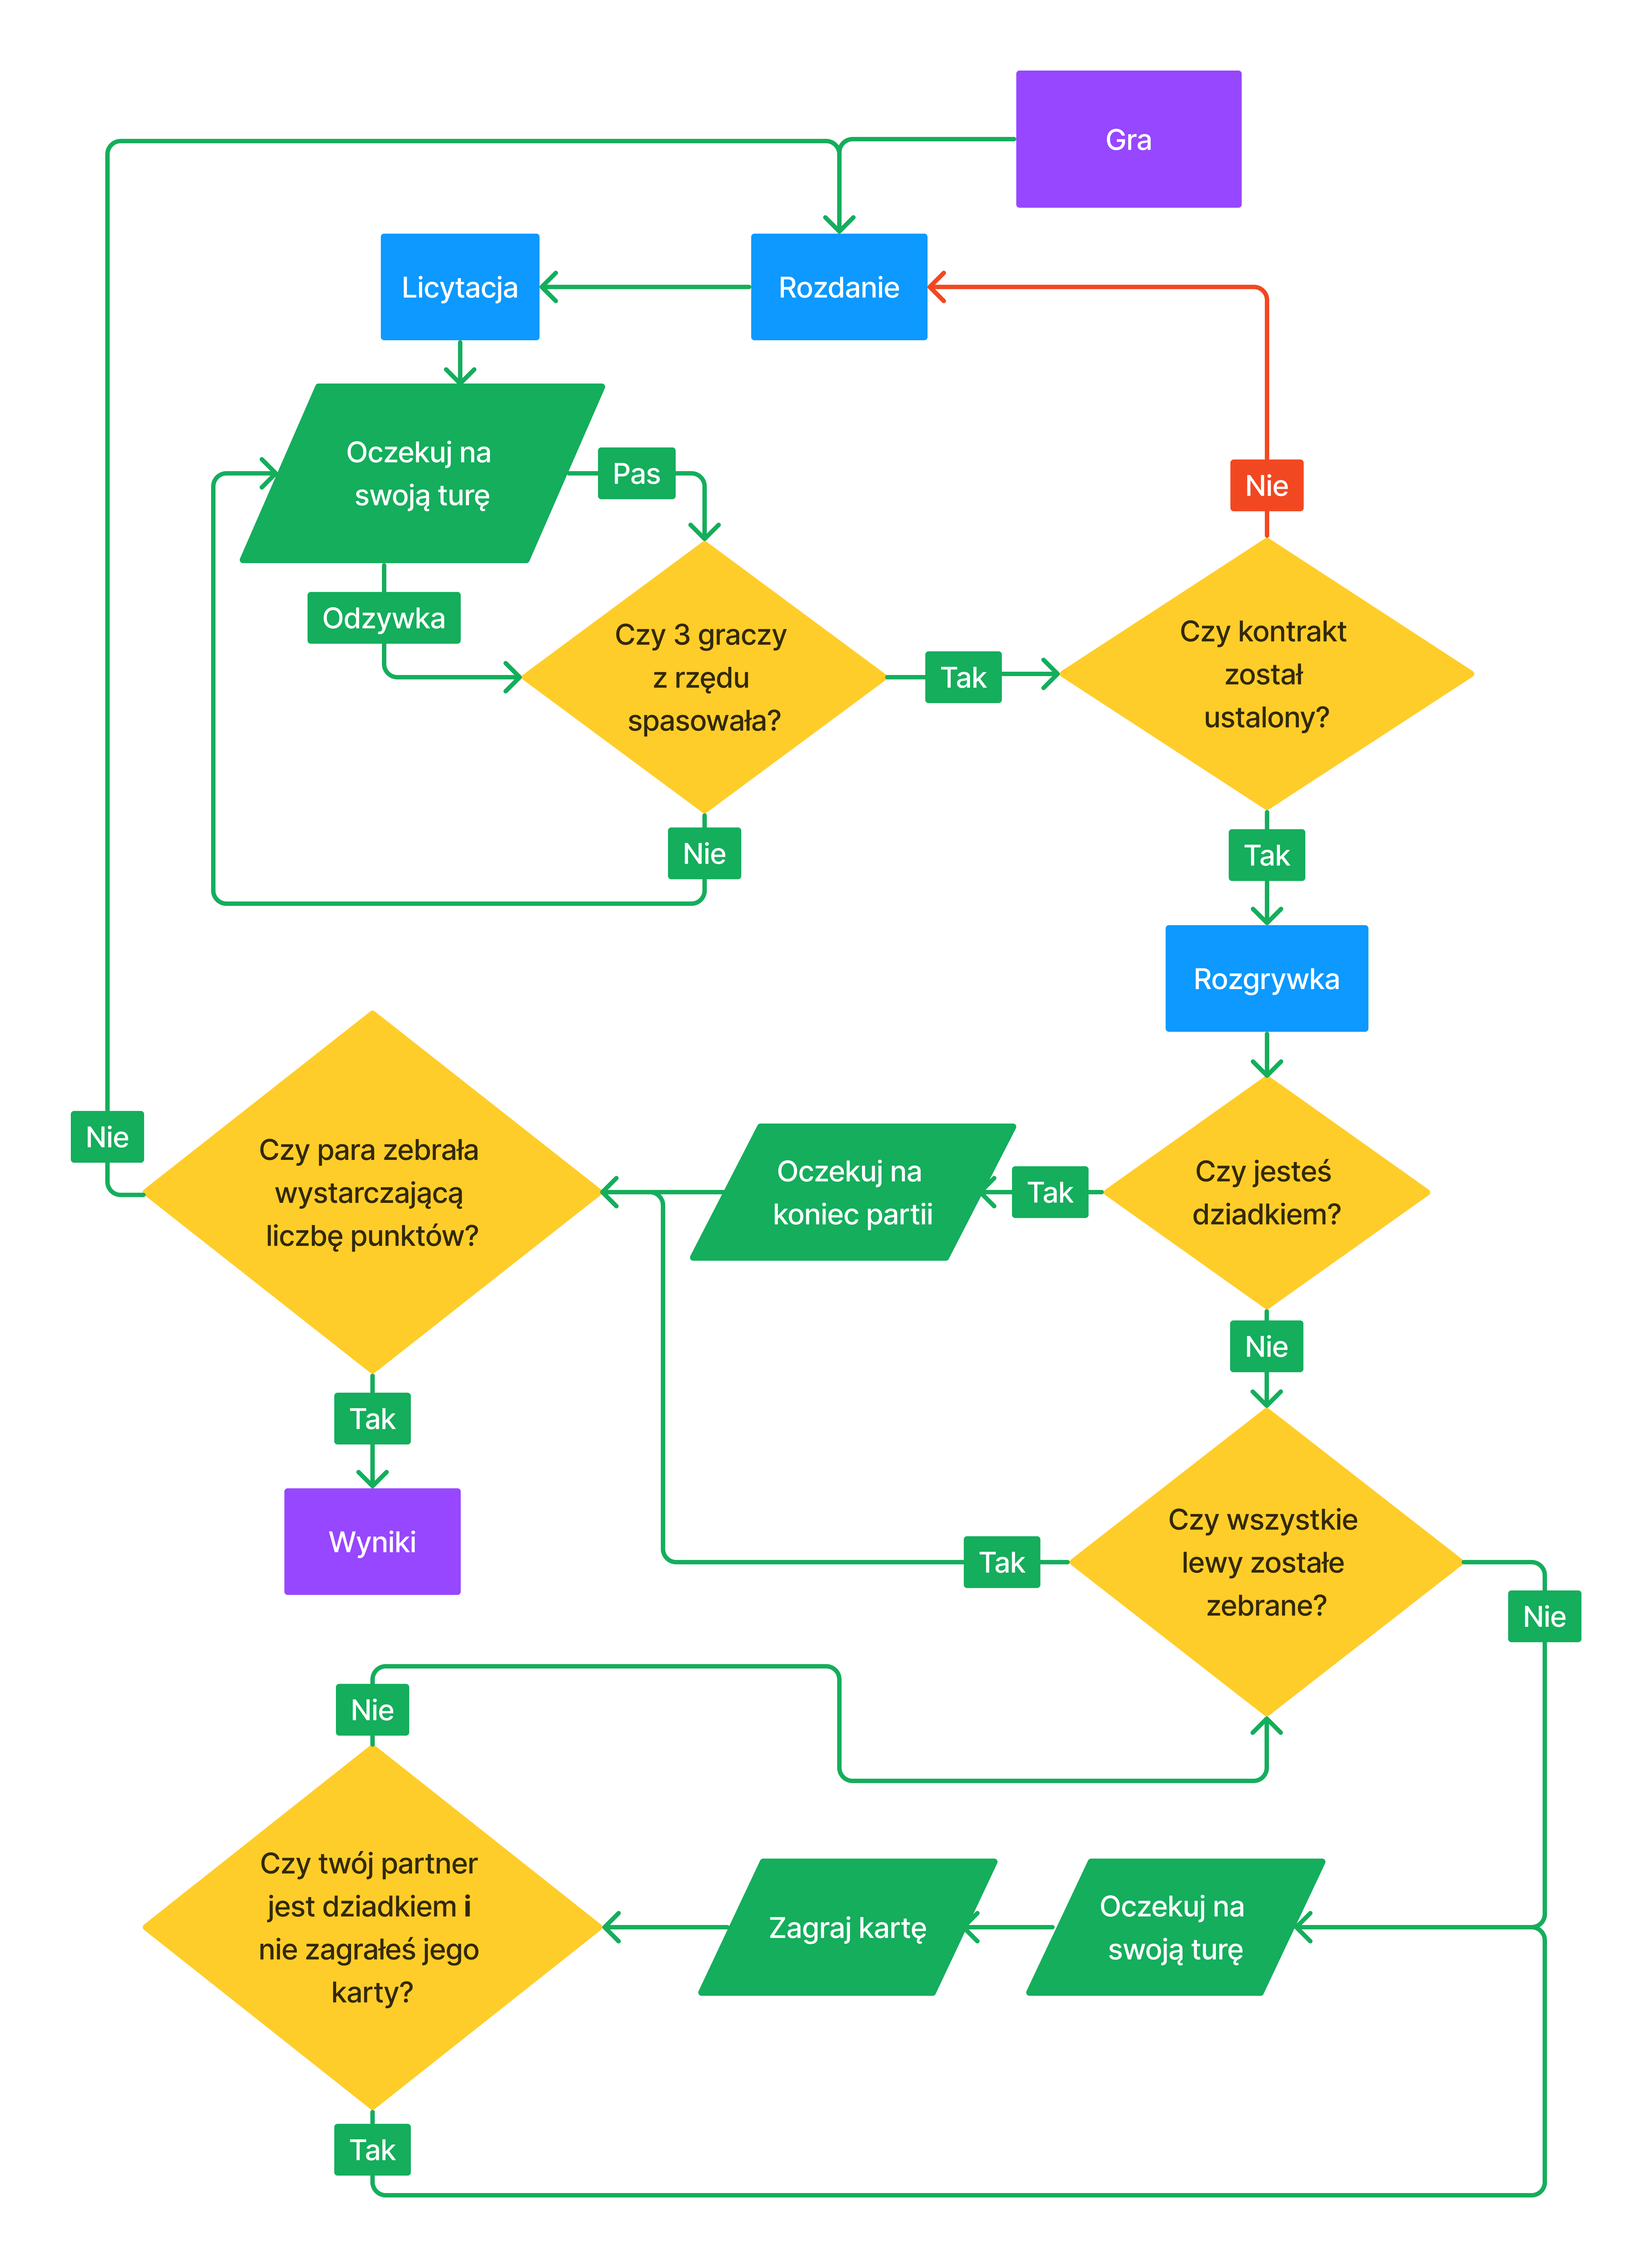
\includegraphics[width=\textwidth]{img/flow-aplikacji/game_flow.png}
  \caption{Schemat interakcji użytkownika z aplikacją podczas rozgrywki brydża}
\end{figure}

\FloatBarrier

\section{Przypadki użycia}

\subsection{Rejestracja/Logowanie do aplikacji}

Aby uzyskać dostęp do większości funkcjonalności aplikacji, wymagane
jest posiadanie konta. Anonimowy użytkownik może je utworzyć, klikając
opcję "\textbf{Register}" w~nagłówku strony. Po kliknięciu użytkownik
zostanie przekierowany do formularza rejestracyjnego.
Do utworzenia konta wymagane jest podanie własnego
pseudonimu, adresu e-mail oraz hasła. Aby uzyskać dostęp do utworzonego
konta, należy kliknąć "\textbf{Log in}" w~nagłówku strony, po czym
w~formularzu podać dane wykorzystanie podczas rejestracji.

W~przypadku nieprawidłowo podanych danych podczas rejestracji
lub logowania, błędów wynikających z~połączeniem internetowym lub
niedostępnym serwerem autentykacji użytkownik otrzyma odpowiednią
informację na ekranie.

\begin{figure}[h]
  \centering
  \includegraphics[width=\textwidth]{example-image-a}
  \caption{}
\end{figure}

\FloatBarrier

\subsection{Tworzenie lobby}

Rozpoczęcie gry w~brydża jest dostępne z~poziomu lobby. Aby utworzyć
lobby, należy kliknąć "\textbf{Create lobby}" na głównym panelu
aplikacji. Przekieruje ono użytkownika do nowego lobby
z~unikalnie wygenerowanym identyfikatorem, którego staje
się administratorem. Użytkownik może udostępnić link do adresu strony,
na której się znajduje, aby udostępnić, np. znajomym swoje lobby, do
którego mogą dołączyć.


\begin{figure}[h]
  \centering
  \includegraphics[width=\textwidth]{example-image-a}
  \caption{}
\end{figure}

\FloatBarrier

\subsection{Dołączanie do lobby}

Gdy użytkownik otrzyma link do lobby od innego użytkownika, może się
do niego dołączyć, wykorzystując adres strony lobby lub wklejając
identyfikator lobby w~odpowiednie pole w~głównym panelu aplikacji
i~klikając opcję "\textbf{Join}". W~obu przypadkach użytkownik zostanie
przekierowany do lobby.

\begin{figure}[h]
  \centering
  \includegraphics[width=\textwidth]{example-image-a}
  \caption{}
\end{figure}

\FloatBarrier

\subsection{Zarządzanie lobby}

Jeżeli użytkownik jest administratorem lub został jedynym
ludzkim graczem w~lobby, może on zarządzać graczami znajdującymi się
wewnątrz. Posiada on następujące możliwości:
\begin{itemize}
  \item usunięcie gracza z lobby -- gracz opuszcza lobby i~nie będzie
        mógł już ponownie do niego dołączyć,
  \item przyznanie pozycji w lobby jako AI -- wybrana pozycja
        gracza w~brydżu będzie kontrolowana przez asystenta AI
        i~uczestniczyć w~rozgrywce jako partner lub przeciwnik,
  \item zamknięcie lobby -- jeżeli administrator jest ostatnim ludzkim
        graczem w~lobby, opuszczenie go spowoduje jego automatyczne
        zamknięcie.
%  \item zmiana statusu lobby na publiczne/prywatne -- powoduje
%         dostępność rozgrywki rozpoczętej przez lobby w~panelu

\end{itemize}

\begin{figure}[h]
  \centering
  \includegraphics[width=\textwidth]{example-image-a}
  \caption{}
\end{figure}

\FloatBarrier

% \subsection{Obserwowanie rozgrywek}

% Gdy jakaś rozgrywka w~brydża została rozpoczęta i~ma ona status
% publiczny, jest możliwe obejrzenie jej z~panelu \textbf{Watch}.
% Z~listy publicznych rozgrywek należy wybrać interesującą i~kliknąć
% ikonę oka. 
% \end{itemize}

% \begin{figure}[h]
%   \centering
%   \includegraphics[width=\textwidth]{example-image-a}
%   \caption{}
% \end{figure}

% \FloatBarrier


\section{Specyfikacja wymagań funkcjonalnych}
Aplikacja nie tylko powinna być dobrze zaprojektowana i wygodna w użyciu, ale także funkcjonalna. Musi spełniać założone wymagania, udostępniając odpowiednie funkcjonalności, żeby była przydatna dla jej użytkowników. Nie da się używać wirtualnego asystenta do gry w brydża, jeśli brakuje w nim asystenta AI, czy w ogóle elementu rozgrywki. Bez spełnienia kluczowych wymagań funkcjonalnych, aplikacja praktycznie nie istnieje. W tym podrozdziale przedstawiamy te wymagania.
\subsection{Logowanie i rejestracja nowych użytkowników}
Żeby uzyskać dostęp do funkcjonalności naszej aplikacji potrzebne jest posiadanie konta i bycie zalogowanym. Dlatego koniecznością jest umożliwienie użytkownikom utworzenia konta, logowania się na nie i późniejszego wylogowania. Formularz rejestracji wymaga podania adresu e-mail, nazwy użytkownika i hasła. Logowanie odbywa się poprzez wprowadzenie swojego adresu e-mail i hasła.
\subsection{Utworzenie/Dołączenie do lobby}
W celu rozegrania partii brydża przeciwko innym graczom, bądź przeciwnikom AI gracz musi mieć możliwość utworzenia własnej rozgrywki oraz dołączenia do istniejącej. Utworzyć jak i dołączyć do lobby można z widoku głównego aplikacji.  Dołączenie do lobby odbywa się poprzez wprowadzenie identyfikatora gry lub wejście w link otrzymany od założyciela lobby. Po utworzeniu lobby użytkownik może wysłać jego identyfikator innym graczom, zapraszając ich do dołączenia, albo zdecydować się wypełnić brakujące miejsca asystentami AI. 
\subsection{Wyrzucenie gracza z lobby}
Administrator lobby może w dowolnym momencie arbitralnie wyrzucić każdego z pozostałych graczy.
\subsection{Rozpoczęcie rozgrywki}
Kiedy do lobby dołączą wszyscy gracze lub część miejsc zostanie obsadzonych asystentami AI, administrator lobby może rozpocząć rozgrywkę, używajac odpowiedniego przycisku. Wszyscy gracze zostają przeniesieni do ekranu gry. 
\subsection{Rozgrywka}
Głównym celem i podstawową funkcjonalnością naszej aplikacji jest rozgrywka w brydża. Każda runda zaczyna się od licytacji, po której gracze wykładają karty zgodie z zasadami gry. Gra kończy się kiedy jedna z par zdobędzie wystarczającą liczbę punktów. Po skończonej rozgrywce użytkownikowi wyświetlany jest ekran z wynikami.
\subsection{Wyświetlenie wyników}
Ważne jest, żeby gracze po skończeniu partii mogli zobaczyć podsumowanie całej rozgrywki. Użytkownikowi wyświetlany jest ostateczny wynik gry, a także liczbę zdobytych przez jego zespół lew oraz możliwych do zdobycia w każdej z rund. Dzięki temu gracze mogą dokładniej przeanalizować rozegraną partię i lepiej oceniać swoje możliwości podczas licytacji w przyszłych rozgrywkach. 
\subsection{Opuszczenie rozgrywki}
Użytkownik może nie tylko wyjść z lobby, ale także w dowolnym momencie opuścić rozgrywkę. W takim przypadku gracz zostaje przeniesiony do ekranu z dotychczasowymi wynikami, a jego miejsce zajmuje asystent AI.
% TODO

\section{Specyfikacja wymagań niefunkcjonalnych}
W naszym projekcie aplikacji - wirtualnego asystenta do gry w brydża, istotą jest zapewnienie nie tylko wszystkich potrzebnych wymagań funkcjonalnych, ale także wygodnej i przyjemnej rozgrywki oraz korzystania z reszty funkcjonalności. Niewiele osób będzie chętnie korzystać z aplikacji, choćby miała ona wyjątkowo rozbudowane spektrum funkcji, jeśli jej działanie będzie niestabilne i pozbawione intuicyjności. W tym podrozdziale przedstawiamy wymagania niefunkcjonalne aplikacji, które są równie ważne jak zdefiniowane wcześniej wymagania funkcjonalne.
\subsection{Dostępność}
Rozwijany przez nas wirtualny asystent do gry w brydża jest aplikacją webową. Dzięki temu będzie on dostępny zarówno dla użytkowników Windows, MacOS, Linux, czy innych systemów operacyjnych. Co więcej, starannie zaprojektowane interfejsy użytkownika (UI) zostały dostosowane tak, aby były wygodne i funkcjonalne nawet na urządzeniach o niewielkich rozmiarach ekranu, umożliwiając płynne korzystanie z aplikacji również na urządzeniach mobilnych.
\subsection{Użyteczność}
Priorytetem naszej aplikacji jest zapewnienie łatwości obsługi i zrozumiałości. Niezwykle istotne jest, aby interfejs użytkownika był intuicyjny, estetyczny i nie zniechęcał potencjalnych użytkowników, ani nie utrudniał korzystania z aplikacji. Dlatego podczas projektowania interfejsu użytkownika kierowaliśmy się zasadami dobrego UI/UX. Stworzyliśmy minimalistyczny i uporządkowany interfejs, który eliminuje chaos i zapewnia spójność na wszystkich podstronach aplikacji. Wykorzystaliśmy ikony o jednakowym znaczeniu na wszystkich stronach, co ułatwia nawigację. Dodatkowo, zastosowaliśmy stałą gamę starannie dobranych kolorów dla elementów interfejsu, co pozwoliło nam utrzymać spójny styl podczas projektowania kolejnych widoków. Aplikacja oferuje tryb jasny i ciemny, aby użytkownicy mogli wygodnie korzystać z niej w zależności od preferencji lub pory dnia. Ponadto, wszystkie podstrony są responsywne, co oznacza, że elementy interfejsu zachowują pełną funkcjonalność, niezależnie od zmiany rozmiaru ekranu, na którym są wyświetlane.
\subsection{Niezawodność}
Wirtualny asystent do gry w brydża tworzony jest z myślą o nauce i doskonaleniu umiejętności, ale także konkurencji i wzajemnym rozgrywkom pomiędzy graczami. Konieczne jest więc wprowadzenie logiki gry z największą dokładnością. Błędy w działaniu aplikacji podczas rozgrywki mogłyby wpłynąć na wynik gry oraz wprowadzić nowych graczy w zakłopotanie, a bardziej doświadczonych w stan irytacji. Niezwykle istotne jest również uniknięcie sytuacji, w których dochodziłoby do utraty połączenia lub braku synchronizacji pomiędzy graczami. Takie incydenty mogą zrujnować całą rozgrywkę i zdecydowanie obniżyć wartość jednej z kluczowych funkcjonalności aplikacji, jaką jest możliwość rozgrywania partii między użytkownikami. Pierwszym krokiem w stronę niezawodności aplikacji było wybranie odpowiednich technologii do jej realizacji. Next.js oraz FastAPI to godne zaufania, popularne na całym świecie narzędzia do budowy aplikacji webowych, a usługa Google Firebase odciąża nas z implementacji funkcjonalności gromadzenia danych i obsługi użytkowników od podstaw. Mając odpowiedni stos technologiczny przystąpiliśmy do implementacji kolejnych funkcjonalności z najwyższą starannością. 

% TODO
